\appendix
\chapter{Appendix}
\begin{figure}
    \centering
	\pgfplotstableread[col sep=semicolon,]{graphs/freezedualmse.csv}\datatable
	\begin{tikzpicture}
	\begin{axis}[
		grid=both,
	    height=7cm,
	    width=\textwidth,
	    legend style={at={(0.95,0.45)},anchor=south east},
	    xtick={0,0.1,...,1},
	    ylabel={Spectral angle (degrees)},
	    xlabel={Dual MSE $\lambda$}]
	    
	    \addplot table [x={lmbda}, y={sangle_test}, 
	    restrict expr to domain={\thisrow{model_id}}{1:1}]{\datatable};
	    \addlegendentry{Combined-AllFrozen}
	    
	    \addplot table [x={lmbda}, y={sangle_test}, 
	    restrict expr to domain={\thisrow{model_id}}{2:2}]{\datatable};
	    \addlegendentry{Combined-EncoderFrozen}
	    
	    \addplot table [x={lmbda}, y={sangle_test}, 
	    restrict expr to domain={\thisrow{model_id}}{3:3}]{\datatable};
	    \addlegendentry{FastCombined-AllFrozen}
	    
	    \addplot table [x={lmbda}, y={sangle_test}, 
	    restrict expr to domain={\thisrow{model_id}}{4:4}]{\datatable};
	    \addlegendentry{FastCombined-EncoderFrozen}
	    
	    \addplot table [x={lmbda}, y={sangle_test}, 
	    restrict expr to domain={\thisrow{model_id}}{5:5}]{\datatable};
	    \addlegendentry{FastCombined-NothingFrozen}
	\end{axis}
	\end{tikzpicture}
	\caption[Dual MSE Loss Analysis (Spectral Angle)]{Dual MSE lambda plot}
	\label{fig:dualmselossangle}
	\end{figure}
	
%\begin{figure}
%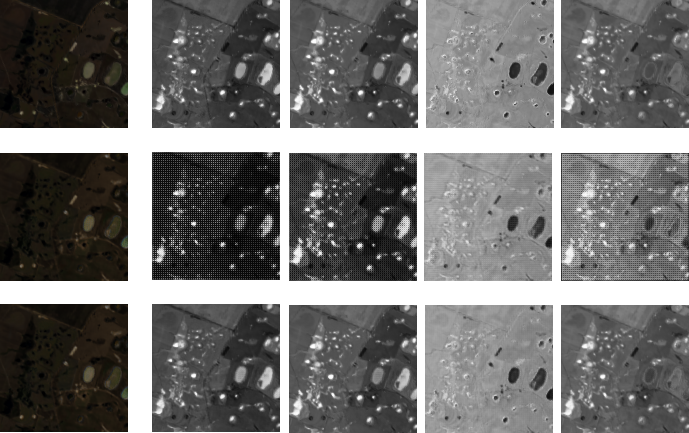
\includegraphics[scale=0.65]{img/latents.png}
%\caption{Latent image comparison}
%\label{fig:latentcompare2}
%\end{figure}
\endinput